\documentclass[12pt,a4paper]{article}
\usepackage{fontspec, xunicode, xltxtra}
\setmainfont{SimSun}
\usepackage{indentfirst} 
\setlength{\parindent}{2em}
\XeTeXlinebreaklocale "zh"
\usepackage[left=2.5cm,right=2.5cm,top=2.5cm,bottom=2.5cm]{geometry}
\usepackage{changepage}
\usepackage{float}
\usepackage{setspace}
\usepackage{amsmath}
\usepackage{amsfonts}
\usepackage{amssymb}
\usepackage{circuitikz}
\usepackage{graphicx}
\usepackage{listings}
\usepackage{color}
\lstset{
language=Verilog,
breaklines=true,
numbers=left,
frame=single,
keywordstyle=\color[rgb]{0,0,1},
commentstyle=\color[rgb]{0.133,0.545,0.133},
stringstyle=\color[rgb]{0.627,0.126,0.941},
xleftmargin=1cm,
xrightmargin=1cm,
aboveskip=1cm
}
\title{实验五\quad 正弦波峰-峰值的测量和显示}
\author{自54 田毅\\ 2015011451}

\graphicspath{{Figure/}}
\begin{document}
\begin{spacing}{1.3}
\maketitle
\tableofcontents
\newpage
\section{实验目的}
\begin{enumerate}
\item 以数字化测量电路为例,熟悉小型电子系统的设计和实现;
\item 体会模块化设计思路,学习单元电路的合理选择;
\item 进一步熟练掌握基于Multisim的电路参数辅助设计和电路功能、性能仿真;
\item 进一步训练电子电路的安装和调试方法;
\item 体会电子系统性能指标的评估及改善方法。
\end{enumerate}
\section{电路框图设计及各模块简略说明}
电路的结构框图如下所示:
\begin{figure}[H]
\centering
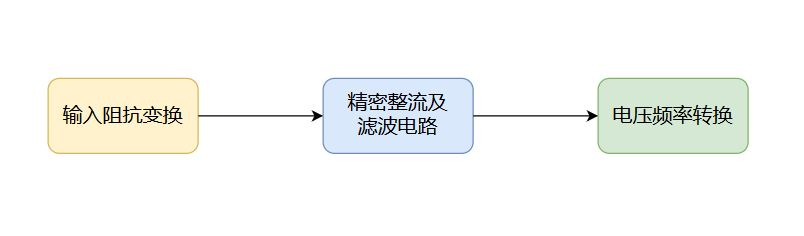
\includegraphics[width=\textwidth]{0.jpg}
\end{figure}
对此作出说明如下。
\begin{enumerate}
\item 输入信号应先经过电压跟随器或反相比例放大器进行预处理,既能满足较大的输入电阻又能实现切换量程的功能。
\item 此后经过全波精密整流电路和滤波电路,将正弦波转换为与其有效值成正比的直流电压。
\item 再经过电压-频率转换电路,将直流电压转换成频率与其值成正比的矩形波信号。
\item 最后使用编程用于频率测量的FPGA显示出频率,及正弦波的峰-峰值。
\end{enumerate}
\section{单元电路的选择和参数设计过程}
\subsection{全波精密整流及滤波电路}
\begin{figure}[H]
\centering
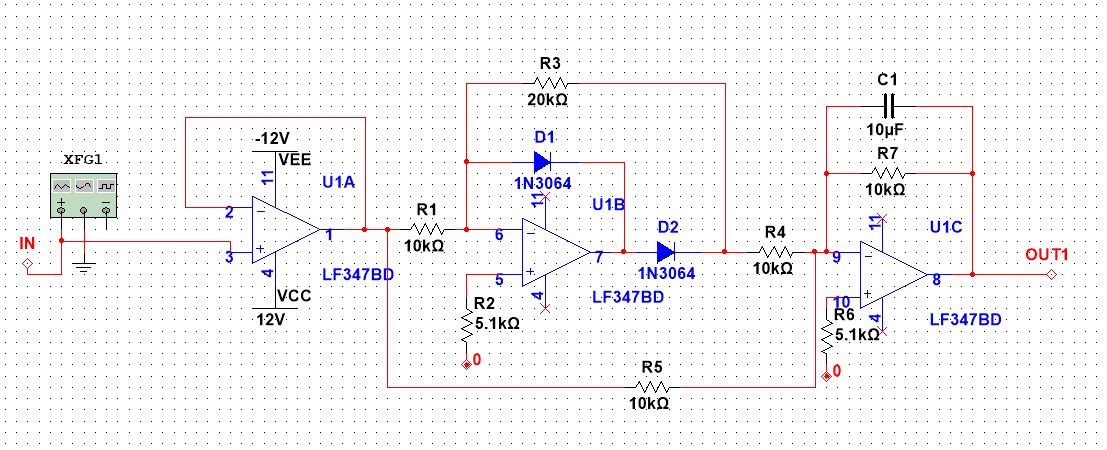
\includegraphics[width=\textwidth]{1.jpg}
\end{figure}
要求量程为$1V\sim 5V$。可通过放大倍数为1的反相比例运算器,然后信号经过全波精密整流电路,相当于取绝对值,并根据电阻$R_7和R_4$的比例改变输出的幅值。\par
为简化电路,在实现全波整流的同时实现滤波,将全波整流电路的第二级(用于反相相加)的反馈网络出直接并联一个电容$C_1,和R_6$构成低通滤波电路。可以看到,这种设计可以节省一个运算放大器的使用,这种优势在后来实际搭电路时得到显现。\par 计算截止频率
\[f_0=\frac{1}{2\pi C_1 R_6}=\frac{1}{2\pi \times 10\mu F \times 10k\Omega} \approx 1.6Hz\]
而输入信号的频率为$20Hz\sim 200Hz$,可见全波整流所得信号的基频分量也几乎无法通过,故此部分的电路输出几乎只有直流分量。\par 仿真中结果如下。
\begin{figure}[H]
\centering
\includegraphics[width=\textwidth]{1+.jpg}
\end{figure}
可以看到,输入为幅值$1V$正弦波时,输出电压$-633mV$左右,波动幅值约$3mV$,仅为$0.5\%$,这说明参数设计合理。\par 
为实现反相全波整流,图中两个二极管方向均与书中相反。输入正弦电压的峰-峰值与输出直流电压的关系为:
\[U_{OUT1} = \frac{U_I}{\pi} \cdot \frac{R_7}{R_4} \approx 0.318 U_I\]
仿真中验证了两者线性关系很好,同时$U_{OUT1}<0$。
\subsection{电压-频率转换电路}
\begin{figure}[H]
\centering
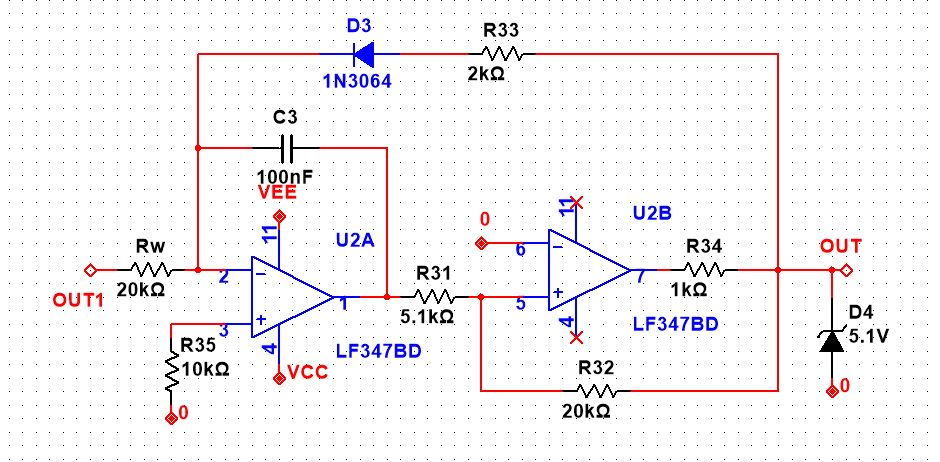
\includegraphics[width=\textwidth]{2.jpg}
\end{figure}
此电路通过积分器和滞回比较器组成了压控振荡电路。若$R_w>>R_{33}$,则此部分电路将上一级输出的直流电压转换成频率与其值近似成正比的矩形波。考虑到下一级的输出为FPGA,故输出端需从两个齐纳二极管改造为并联一个齐纳二极管,使得输出高低电平分别为$U_H=5.1V$,$U_L=-0.7V$左右,从而满足后级的要求。通过计算可得频率与输入电压的关系:
\[
f_{OUT} = \frac{R_{32}}{R_{31} R_w C_3(U_H-U_L)} \cdot U_{OUT1} \approx 338.1 U_{OUT} \approx 107.6 U_I
\]
故$U_I$介于$1V\sim 5V$时,$f_{OUT}$大约为$107.6Hz\sim 538.1Hz$。实际电路搭建中,通过精密调节$R_w$,当能够使其在$20k\Omega$以上的某个值使得输入峰-峰值$1V$的正弦电压时,输出精确为$100Hz$的矩形波。\par 
输入为峰-峰值$2V$正弦波时,仿真测得输出频率为$193Hz$,基本符合预期,观察到的波形如下:
\begin{figure}[H]
\centering
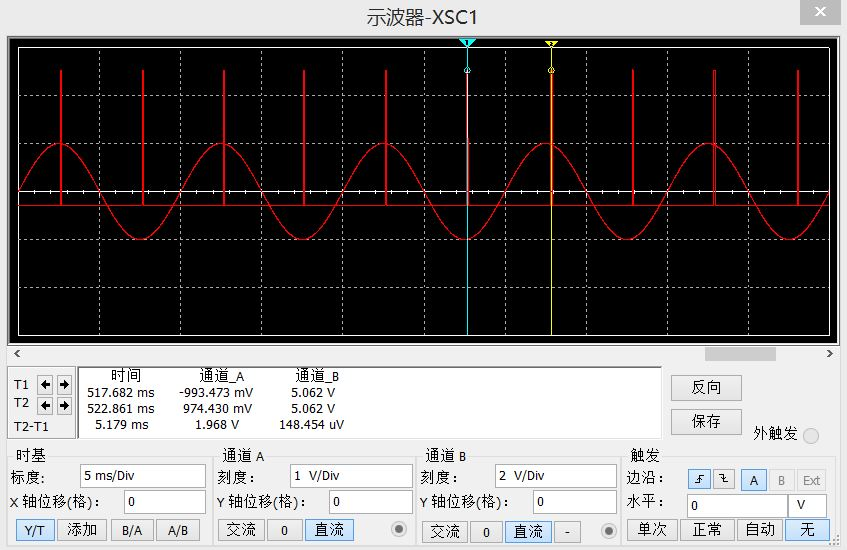
\includegraphics[width=\textwidth]{4.jpg}
\end{figure}
\section{最终电路图、测量结果及测量精度分析}
\subsection{最终电路图}
最终电路图即电路框图中三部分的组合,如下所示。
\begin{figure}[H]
\centering
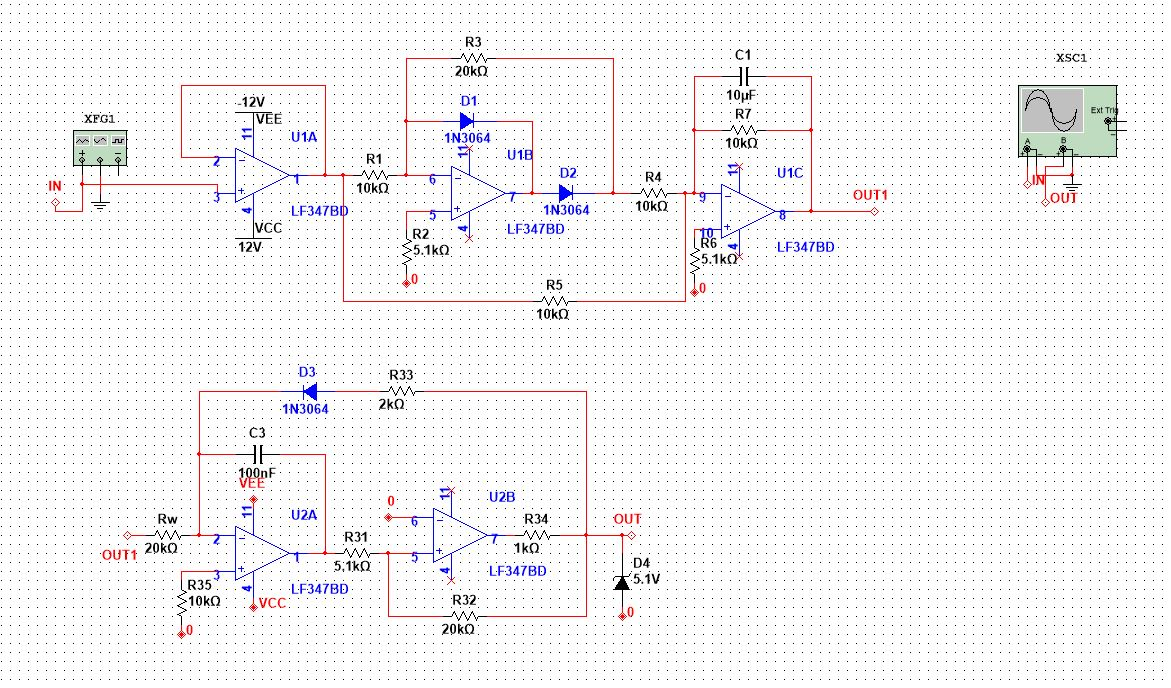
\includegraphics[width=\textwidth]{3.jpg}
\end{figure}
\subsection{$1V\sim 5V$正弦波测量结果及精度分析}
\subsubsection{波形图}
以下是输入峰-峰值$1V\sim 5V$、频率$20Hz\sim 200Hz$的正弦波时的示波器截图。\par 
输入峰-峰值$1V、频率100Hz$的正弦波,输出频率约$100Hz$,波形如下。
\begin{figure}[H]
\centering
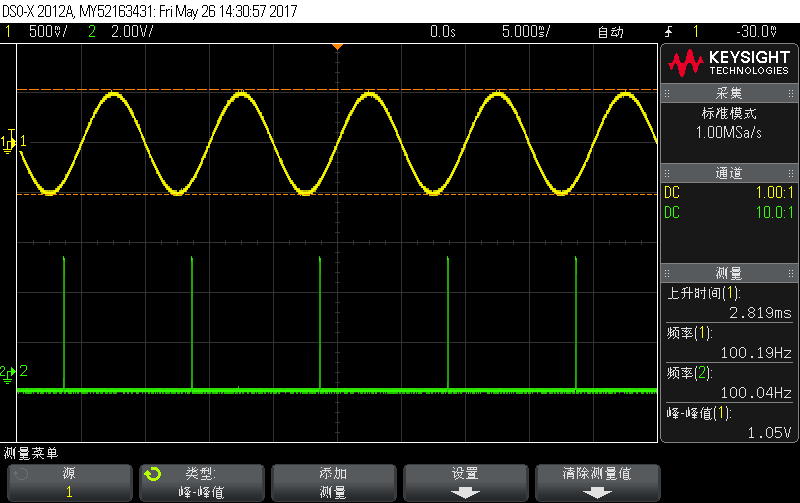
\includegraphics[width=\textwidth]{scope_0.png}
\end{figure}
输入峰-峰值$5V、频率100Hz的正弦波,输出频率约483Hz$,波形如下。
\begin{figure}[H]
\centering
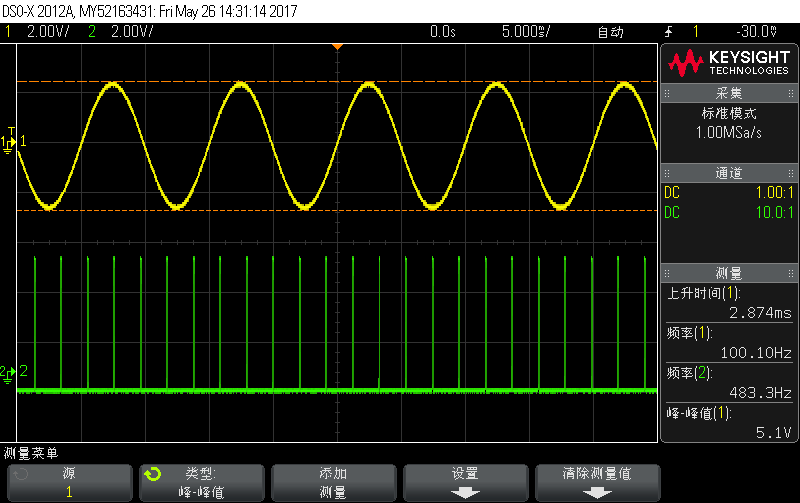
\includegraphics[width=\textwidth]{scope_1.png}
\end{figure}
下面进行是极限频率测试结果。\par 
输入峰-峰值$5V、频率20Hz的正弦波,输出频率约482Hz$,波形如下。
\begin{figure}[H]
\centering
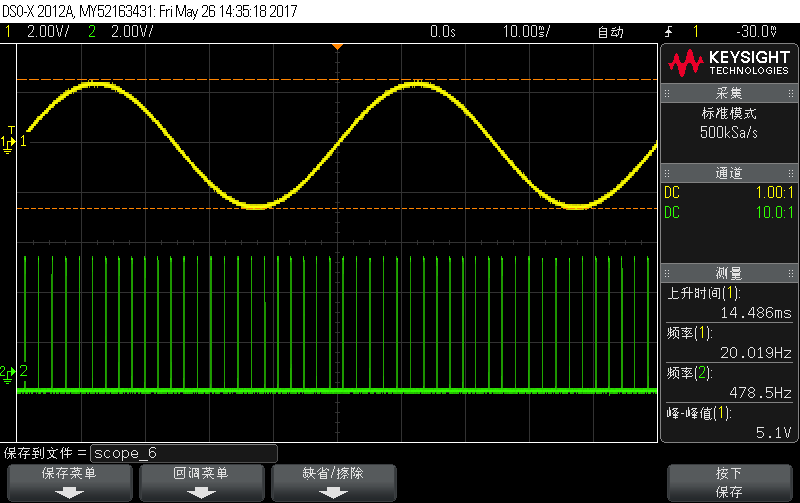
\includegraphics[width=\textwidth]{scope_6.png}
\end{figure}
输入峰-峰值$5V、频率20Hz的正弦波,输出频率约482Hz$,波形如下。
\begin{figure}[H]
\centering
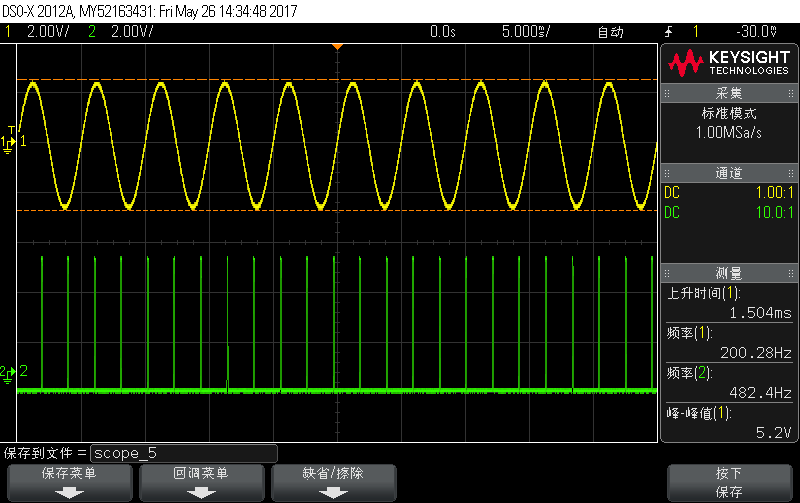
\includegraphics[width=\textwidth]{scope_5.png}
\end{figure}
\subsubsection{FPGA显示数据}
将编程好的FPGA接于输出端,整理FPGA测量结果如下表。
\begin{table}[H]
\centering
\begin{tabular}{|c|c|c|c|c|c|}
\hline 
输入电压峰-峰值$U_{ip-p}/V$&$1.00$&$2.00$&$3.00$&$4.00$&$5.00$\\ \hline 
输入频率$20Hz时输出频率f_{OUT}/10^2Hz$&$100$ &$1.98$ &$2.94$ &$3.90$ &$4.82$ \\ \hline
误差/\%&$0$&$1$&$2$&$2.5$&$3.6$\\ \hline
输入频率$50Hz时输出频率f_{OUT}/10^2Hz$&$1.00$ &$198$ &$2.94$ &$3.90$ &$4.82$ \\ \hline
误差/\%&$0$&$1$&$2$&$2.5$&$3.6$\\ \hline
输入频率$100Hz时输出频率f_{OUT}/10^2Hz$&$1.00$ &$1.98$ &$2.94$ &$3.90$ &$4.82$ \\ \hline
误差/\%&$0$&$1$&$2$&$2.5$&$3.6$\\ \hline
输入频率$150Hz时输出频率f_{OUT}/10^2Hz$&$1.00$ &$1.98$ &$2.94$ &$3.90$ &$4.82$ \\ \hline
误差/\%&$0$&$1$&$2$&$2.5$&$3.6$\\ \hline
输入频率$200Hz时输出频率f_{OUT}/10^2Hz$&$1.00$ &$1.98$ &$2.94$ &$3.90$ &$4.82$ \\ \hline
误差/\%&$0$&$1$&$2$&$2.5$&$3.6$\\ \hline
\end{tabular} 
\end{table}
由上表可见,在所有频率、电压范围内均满足$8\%$的精度要求。实际上精度可达$3.6\%$。而此电路对于各频率电压均有相当好的稳定性,这得益于滤波电路的优越性能。
\subsection{$0.1V\sim 1V$正弦波测量结果及精度分析}
\subsubsection{波形图}
以下是输入峰-峰值$1V\sim 5V$、频率$20Hz\sim 200Hz$的正弦波时的示波器截图。\par 
输入峰-峰值$0.1V、频率100Hz$的正弦波,输出频率约$9.7Hz$,波形如下。
\begin{figure}[H]
\centering
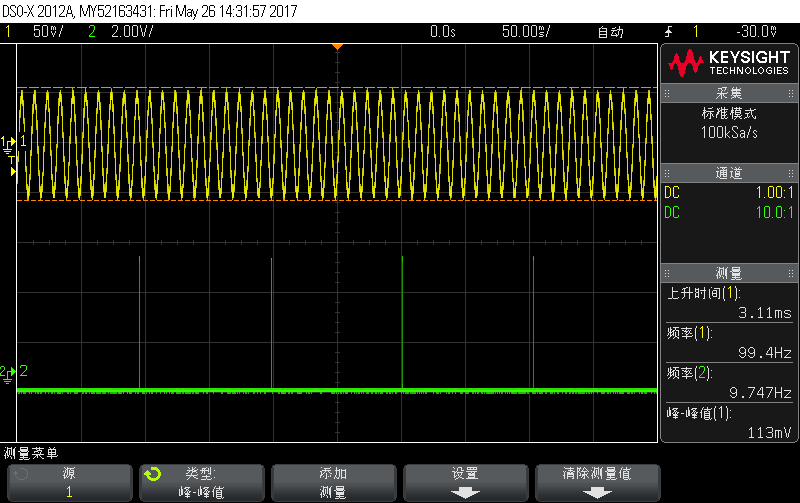
\includegraphics[width=\textwidth]{scope_2.png}
\end{figure}
输入峰-峰值$0.1V、频率20Hz的正弦波,输出频率约9.7Hz$,波形如下。
\begin{figure}[H]
\centering
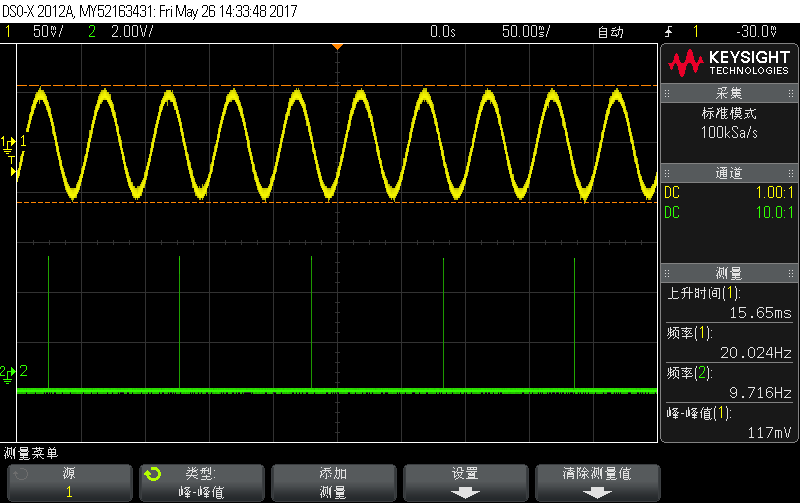
\includegraphics[width=\textwidth]{scope_3.png}
\end{figure}
下面进行是极限频率测试结果。\par 
输入峰-峰值$0.1V、频率200Hz的正弦波,输出频率约9.7Hz$,波形如下。
\begin{figure}[H]
\centering
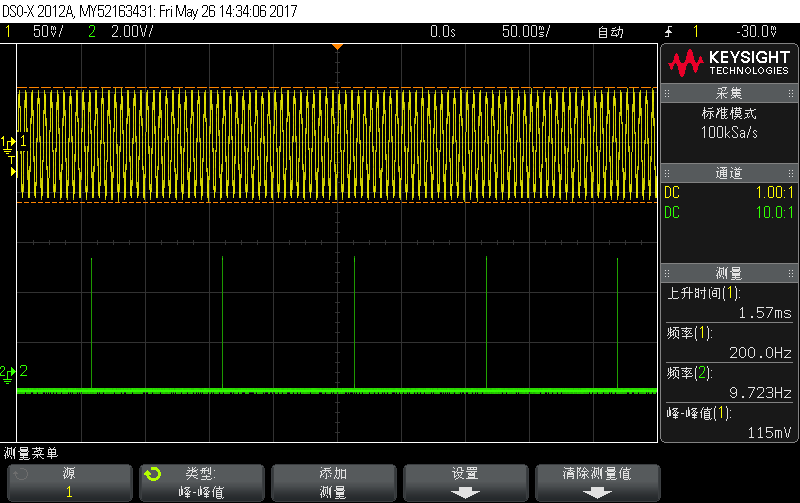
\includegraphics[width=\textwidth]{scope_4.png}
\end{figure}
\subsubsection{FPGA显示数据}
将编程好的FPGA接于输出端,整理FPGA测量结果如下表。
\begin{table}[H]
\centering
\begin{tabular}{|c|c|c|c|c|c|}
\hline 
输入电压峰-峰值$U_{ip-p}/V$&$0.1$&$0.3$&$0.5$&$0.7$&$0.9$\\ \hline 
输入频率$20Hz时输出频率f_{OUT}/10^2Hz$&$0.10$ &$0.30$ &$0.50$ &$0.70$ &$0.90$ \\ \hline
误差/\%&$0$&$0$&$0$&$0$&$0$\\ \hline
输入频率$50Hz时输出频率f_{OUT}/10^2Hz$&$0.10$ &$0.30$ &$0.50$ &$0.70$ &$0.90$ \\ \hline
误差/\%&$0$&$0$&$0$&$0$&$0$\\ \hline
输入频率$100Hz时输出频率f_{OUT}/10^2Hz$&$0.10$ &$0.30$ &$0.50$ &$0.70$ &$0.90$ \\ \hline
误差/\%&$0$&$0$&$0$&$0$&$0$\\ \hline
输入频率$150Hz时输出频率f_{OUT}/10^2Hz$&$0.10$ &$0.30$ &$0.50$ &$0.70$ &$0.90$ \\ \hline
误差/\%&$0$&$0$&$0$&$0$&$0$\\ \hline
输入频率$200Hz时输出频率f_{OUT}/10^2Hz$&$0.10$ &$0.30$ &$0.50$ &$0.70$ &$0.90$ \\ \hline
误差/\%&$0$&$0$&$0$&$0$&$0$\\ \hline
\end{tabular} 
\end{table}
由上表可见,在所有频率、电压范围内仍满足$8\%$的精度要求。实际上精度可达$0\%$。此电路对于小幅值情况下各频率电压仍有相当好的稳定性,这仍得益于滤波电路的优越性能。因此对于选作内容2无需做出电路上的改进。
\section{基于FPGA的频率测量显示模块代码}
\subsection{分频器模块}
分频器模块用于给各模块分频,提供需要的频率,代码如下。
{
\ttfamily
\begin{lstlisting}
module timedivider(
    clk, times, clk_out
);

input clk;
input[31:0] times;
output reg clk_out;

reg[31:0] cnt;//count
initial clk_out = 0;
initial cnt = 0;

always@(posedge clk)
begin
    if (cnt == times - 1 )
    begin
        clk_out <= ~ clk_out;
        cnt <= 0;
    end
    else cnt <= cnt + 1;
end 
endmodule
\end{lstlisting} 
}
\subsection{频率计数模块}
这是本次编程的算法核心模块。在1s的时间内,通过比较当前时刻取样的输入与上一时刻的输入来判断是否到达上升沿,在上升沿计数,1s中上升沿的个数即为频率。代码如下。
{
\ttfamily
\begin{lstlisting}
module fq_cnt(
    clk, in,
    d2, d1, d0
);
input clk, in;//clk = 1Hz, in is the measured signal
output reg [3:0] d2, d1, d0;

//other variables
reg [1:0] clkc = 2'b0;//clock copy
reg [19:0] cnt = 0;//count max is 2^20

always@ (posedge in)
begin
    clkc[1:0] = {clkc[0], clk};
    if (clkc[0] > clkc[1])
    begin
        d0 = cnt % 10; cnt = cnt / 10;
        d1 = cnt % 10; cnt = cnt / 10;
        d2 = cnt % 10;
        cnt = 0;
    end
    cnt = cnt + 1;
end

endmodule
\end{lstlisting} 
}
\subsection{输出模块}
输出模块用于将计数结果显示出来。segments.v(七段数码管)代码如下。
{
\ttfamily
\begin{lstlisting}
module segments(
    clk, d3, d2, d1, d0,
    sel, out
);
 input clk;
 input [3:0] d3, d2, d1, d0;
 output reg [3:0] sel = 4'b1110;//select signal output
 output wire [6:0] out;//segments output
 
 //other variables
 reg [3:0] now;
 
 //scan
 always@ (posedge clk)//shift one digit
     sel <= {sel[2:0],sel[3]};
 
 always@ (sel)
     case( sel )
         4'b1110: now = d0;
         4'b1101: now = d1;
         4'b1011: now = d2;
         4'b0111: now = d3;
         default: now = 4'hf;//for debugging
     endcase
     
 seg_decoder SEG_D0( now, out );
 
endmodule
\end{lstlisting} 
}
其中用到了seg{\_}decoder模块,这是一个译码器模块,用于将十进制数译作数码管上的七段电平信号,代码如下。
{
\ttfamily
\begin{lstlisting}
module seg_decoder(
    in,
    out,    
    );

//describe
input [3:0] in;
output reg [6:0] out;

//always
always@ ( in ) begin
    case( in )
        4'b0000: out = 7'b1000000;
        4'b0001: out = 7'b1111001;
        4'b0010: out = 7'b0100100;
        4'b0011: out = 7'b0110000;
        4'b0100: out = 7'b0011001;
        4'b0101: out = 7'b0010010;
        4'b0110: out = 7'b0000011;
        4'b0111: out = 7'b1111000;
        4'b1000: out = 7'b0000000;
        4'b1001: out = 7'b0010000;
        default: out = 7'b1111111;
    endcase
end
endmodule
\end{lstlisting} 
}
\subsection{顶层模块}
顶层模块完成分频器、频率计数、输出三个模块的调用,代码如下。
{
\ttfamily
\begin{lstlisting}
module fm_top(
    clk, in,
    seg_sel, seg_out
);
input clk, in;//clk = 100MHz, in is measured signal
output wire [3:0] seg_sel;
output wire [6:0] seg_out;

//other variables
//wire in;//256Hz
wire clk0; //1Hz
wire clk_seg;//200Hz
wire [3:0] d2, d1, d0;

//call modules
timedivider
DIV0(clk, 50000000, clk0),//1Hz
DIV_SEG(clk, 250000, clk_seg);//200Hz
//DIV_IN(clk, 195312, in);//256Hz
fq_cnt FC0(clk0, in, d2, d1, d0);
segments SEG0(clk_seg, 0, d2, d1, d0, seg_sel, seg_out);

endmodule
\end{lstlisting} 
}
由于代码均已配有详细注释,在此不再对代码含义赘述。
\section{实验中遇到的问题及解决方法}
本次实验准备非常充分,代码已经过仿真测试,鲁棒性很好;在实验课之前电路已提前在面包板搭好,并已用mydaq进行测试;因此,实际上在实验课上没有遇到困难。遇到的问题主要在代码编写过程与仿真过程中。
\subsection{同一变量不能在两个always语句中赋值的问题}
在编写完程序进行仿真时,报错显示不能对于一个变量在两个always触发下都进行赋值操作。这就使得,直接使用输入信号的上升沿触发使计数器自增,再在$1Hz$信号上升沿触发下计数器清零的想法不能实现。由于输入信号最低频率$20Hz > 1Hz$,所以仍使用输入信号上升沿触发,而将对时钟信号的上升沿检测改为比对当前对$1Hz$时钟的取样值与上一触发时的取样值的差异。这样在一个always中即解决了问题。事实证明,这种方式具有很好的鲁棒性。
\subsection{仿真成功Implementation却报错的问题}
最初使用内置信号源进行测试后,改用外部引脚的信号作为输入进行测试。但是,在仿真无误的情况下,却出现了implementation阶段报错的奇怪问题。经过与同学的讨论,这一问题的原因在于,使用的vivado软件认为不能在默认情况下使用外部信号作为触发源,为此,需要在constraints文件中加一行:
{
\ttfamily
\begin{lstlisting}
set_property CLOCK_DEDICATED_ROUTE FALSE [get_nets in_IBUF]
\end{lstlisting} 
}
这个问题的解决花费了大量时间,但也通过调试这个bug对于vivado下各文件之间的关系有了更好的理解。
\subsection{将两个齐纳管换为一个后电路不起振的问题}
在做仿真时,大体进行逐级调试,因此遇到的问题总能及时发现并解决。但在最后,当将两个齐纳管换为一个后电路不起振的问题困扰了我很久。\par 
首先,我尝试了在两个齐纳管的输出以后再串接一个$1k\Omega$的电阻再接一个齐纳管的方式。发现不论此时齐纳管正负极方向如何,都能得到符合预期的$-0.7V\sim 5.1V或-5.1V\sim 0.7V$的结果。但如此,在输出环节需要三个齐纳管,在我并不满意的。\par 
后来,我认真地研究了电路的原理,并在和同学的讨论中,发现将这个压控振荡电路的二极管或这个齐纳管的正负极对调即可解决问题。这正是电路起振的原理决定的:若二极管与单个齐纳管的正负极不匹配,则在齐纳管正向导通时无法使二极管导通,因此无法“电荷平衡”,自然不可能起振。由于输出要求$-0.7V\sim 5.1V$,我最后选择了颠倒二极管的正负极方向。但这样一来,要求输入的直流电压就由正变负,为此特意更改了全波整流及滤波电路中的两个二极管方向,实现了反相全波整流及滤波。
\subsection{电容正负极性的判断}
这是在搭实际电路时遇到的一个小问题。实际中$10\mu F$电容是一个电解电容,需要确定正负极。一方面,可以通过理论分析获知;而本次实验中,采用了仿真的方式确定,快捷而顺利地解决了这一问题。这体现出EDA的优越性。
\section{实验体会}
这次实验FPGA选做验收在实验室上电后立刻调试完毕,而正弦波峰-峰值的测量在上电后也立刻得到了稳定、准确的结果,因此是非常顺利的一次实验。本次实验实际上是一个小型电子系统的设计和实现过程,在成功实现的过程中感我也感受到莫大的喜悦。经过这次实验,我主要有以下四点体会。
\begin{enumerate}
\item 首先,初步体会到分模块设计的重要性。这不仅使得每一步的聚焦点缩小,能够把握,而且为仿真与实际电路调试都带来了巨大的方便。不仅对于模拟部分,数字部分的FPGA编程中模块化、结构化也能给代码带来更强的可读性与鲁棒性。
\item 我体会到了EDA仿真的重要性。本次实验实际上也出现了仿真波形不好的情况,由于已经有上次实验仿真的经验,通过缩小步长我很快解决了这一问题并得到了相当好的波形。仿真上的成功给了我在搭电路时的信心,最终果然各个环节参数选择均比较合理,整个电路能够适应多种情况下正弦波峰-峰值的测量。
\item 我感知到理论与实际的偏差。本次实验要求精度为$\pm 8\%$,仿真、硬件实验结果与理论值相比都确有偏差。我认识到设计、选用各种电路时确应考虑其精度,这让我认识到我们在理论课上学习的各种评价指标的有用之处。
\item 我也体会到数模电结合的喜悦。本次实验实际上可看作是一次数模电结合的综合实验。终于有机会,将电路部分两学期来学习的知识整合到一起去使用,这对于第一次有这种体验的人来说无疑是激动人心的。我预先将程序拷入ROM中,因此只要供电,板子即可运转。本次FPGA编程实践中,我的板子相比于其他同学更加鲁棒,这部分是代码的原因,部分是我使用的Basys3实验板的原因。也因此,在测量压控振荡电路的输出频率时,一些同学向我借FPGA进行预测试,以与他们的板子的测量结果进行比对,这令我感到好板子、好代码对于优秀的电子系统的重要性。
\end{enumerate}
\end{spacing}
\end{document}
